\label{ch1}
\chapter{Datacenter networks}
In the last decades,  with the spreading of cloud services accessible to anyone, computing has undergone a remarkable evolution. Encouraged by the astonishing growth of virtualization technologies in the IT industry, as well as the availability of storage and chips at ever-more modicum prices, over-the-top (OTT) players like Google, Amazon and Microsoft, have been building datacenter hotspots all around the world. Most of the applications any sector of modern society relies on, such as commercial and financial services, Web search, scientific computing, on-demand video streaming, recommendation systems, not to mention social networking and online gaming, more often than not run inside one of their datacenters' infrastructure. Indeed, from small enterprises to large corporations, it has been a common cost-saving strategy to offload, up to a certain extent, the deployment and operation of their own information systems to third parties, the cloud service providers. 
% da dire meglio... voglio dire che diventano providers di servizi non loro
After all, it is well-known in engineering, how much resource concentration enables better design and ease of mantainance.

Among the major challenges posed by cloud computing paradigm, certainly there is the design of a huge communication network, hosting hundreds of thousands of servers, that is required to simultaneously provide high throughput and low-latency, while guaranteeing uninterruptible service continuity and lending itself to relentless expansion.
 The peculiar requirements of the datacenter environment and the lack of flexibility of traditional TCP/IP stack, have pushed the development % exploration
  and adoption of unconventional approaches, such as centralized control and network softwarization (SDN),  laying the premises for a wider transformation process in the network industry. 
In this sense, datacenters can be credited to having represented natural incubators for the evolution of telecommunication networks happening during the last few years. As a matter of fact, virtualization technologies and control plane programmability soon would have become disruptive innovations in networking ecosystem, that started to experience the same changes the IT world faced years before.
%Pushed by datacenters' needs, the research community, both from industry and academia, started to work on innovative solutions that ...  
As a result of this process, nowadays, ISPs are converting their infrastructure towards the same solutions, re-architecting PoPs as small-scaled modern datacenter, with massive employment of virtualization as regards network functions and devices (NFV). Similarly, the next generation mobile network, 5G, is going to base both its core and edge functions on the same paradigm, as revealed by its standardization and by the investments in multi-access edge computing (MEC).


% pervasive extensively widespread make use of massively plenty 


%\section{Datacenter design and management principles}
% dire che è semplice perchè unica entità amministrativa e single location
\section{Interconnection network design}
\label{sec:topology}
The typical structure of a datacenter, as shown in Fig.\ref{fig:dcn},  
is comprised of many \textit{racks}, interconnected among each other thanks to a common network infrastructure. A rack is nothing else than a group of servers physically co-located in a common cabinet, attached to the same \textit{Top of Rack} switch (ToR) and thus  separated by a single hop. In achieving the goal of hosting an enormous amount of servers, the principal bottleneck often results in being the interconnection fabric, usually referred to as \textit{Data Center Network} (DCN). Ideally, it should act as a huge switch, able to provide maximum-rate communication among servers, that is their NIC's access capacity.  At high level, there are fundamentally two ways for practically realizing such infrastructure. The first choice is to rely on complex specialized solutions, like InfiniBand, or high-performance IP devices with many ports, that successfully provide bandwidth for thousands of nodes, however incurring in high deployment and management costs. Conversely, the second possibility is to build the network infrastructure by simply leveraging on commodity off-the-shelf switches that are cheaper, already on economy of scale and fully compatible with existing hardware and operating systems, just as large distributed clusters are made of general purpose cheap computers. This is usually the design pursued by principal cloud providers, as recently disclosed by themselves. A major drawback of the latter strategy, is the difficulty in providing full-rate communication among hosts in different racks. In other words, depending on traffic patterns and especially network topology, it is very hard to place enough inter-rack capacity - usually referred to as \textit{bisection bandwidth} - to satisfy the collective demand of all the racks. 
For this reason, the topology design plays a fundamental role for the feasibility of scalable and cost-beneficial large datacenters. It is worth noticing that sometimes, building a DCN with full bisection bandwidth is unnecessary and cost prohibitive, therefore it is commonly accepted some degree of \textit{oversubscription}, meaning that the ratio between total intra-rack and bisection bandwidth is greater than 1. This choice is acceptable when applications are mostly rack local and statistical multiplexing is beneficial. In general, a non-oversubscribed network allows greater flexibility in resource allocation and deployment of applications across racks, leading to higher utilization which is also important for big cloud providers.
% TODO draw figures of same style
\begin{figure}
	\centering
	\begin{subfigure}[b]{0.45\textwidth}
		\centering
		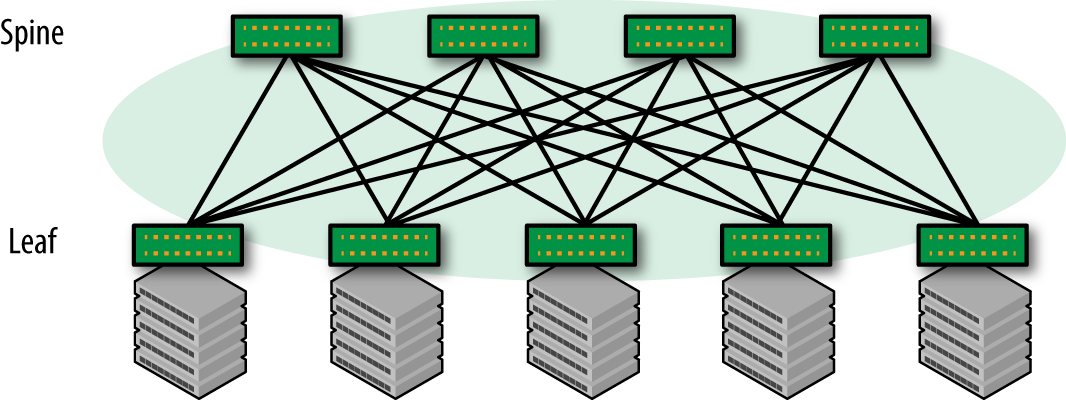
\includegraphics[width=\textwidth]{Chapter1/Figures/leaf-spine}
		\caption{Leaf-Spine}
		\label{fig:leafspine}
	\end{subfigure}
	\hfill
	\begin{subfigure}[b]{0.45\textwidth}
		\centering
		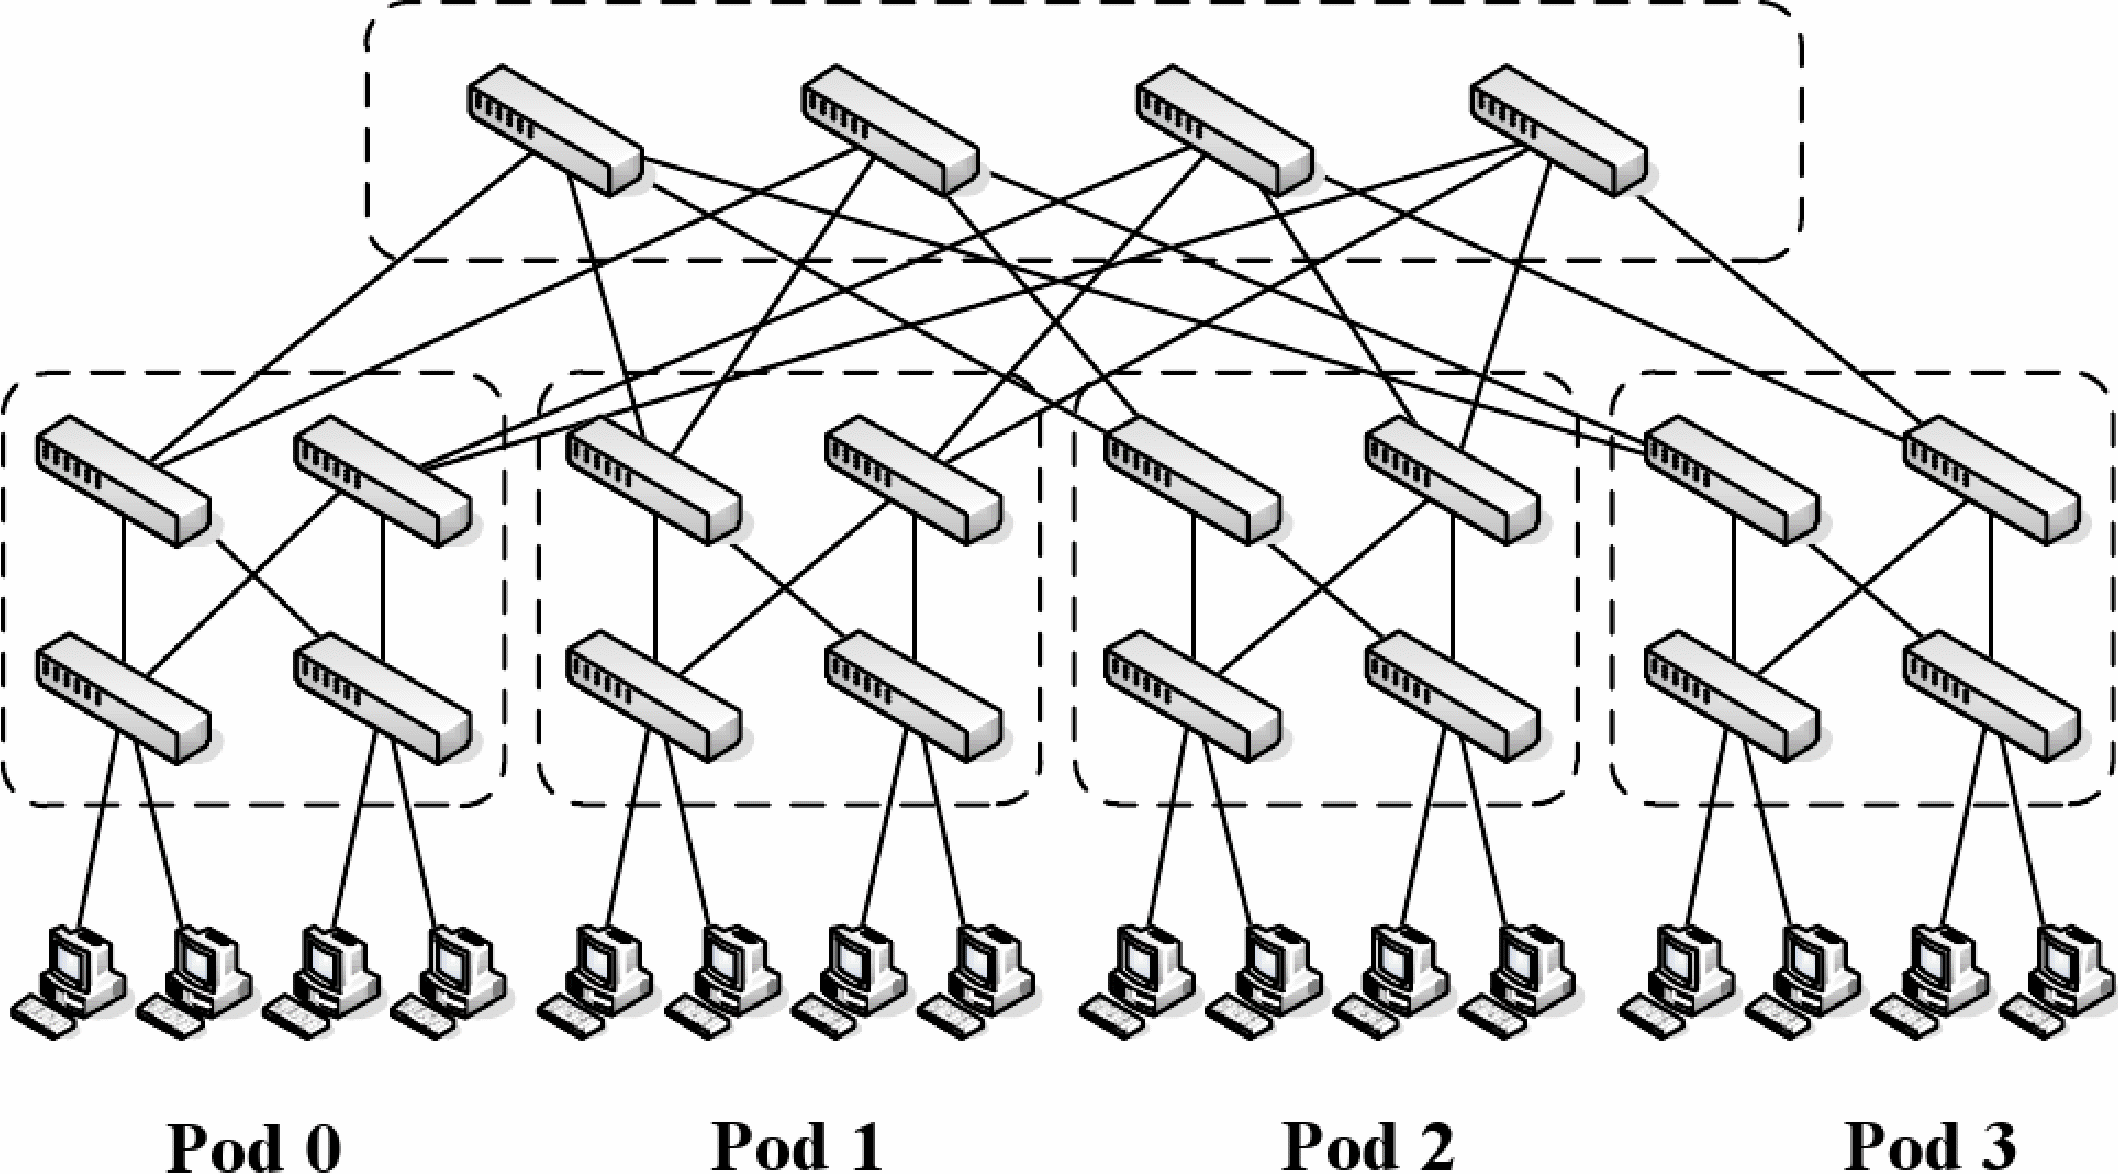
\includegraphics[width=\textwidth]{Chapter1/Figures/fat-tree}
		\caption{3-layers Fat-Tree}
		\label{fig:fattree}
	\end{subfigure}
	\caption{interconnection networks.}
	\label{fig:topology}
\end{figure}

Two examples of topology design are provided in Fig. \ref{fig:topology}.
The \textit{Leaf-Spine} (Fig. \ref{fig:leafspine}), is a typical hierarchical architecture, where the interconnection between leaf and spines switches form a bipartite graph. Despite being popular in campus networks, scaling to thousands of servers would require having spines with lots of high-capacity ports .  
%In general, the desired properties can be summarized in:
%\begin{itemize}
%	
%	\item \textbf{Non-blocking}
%	
%	\item \textbf{Scalable}
%	
%	\item \textbf{Fault tolerant}
%	
%\end{itemize}
A more flexible solution dates back to the early telephone network, when Charles Clos had to solve a similar problem and came up with its proposal for multi-stage switching fabrics. Indeed, the \textit{Fat-Tree} (Fig. \ref{fig:fattree}), representing the most widely adopted topology, is a folded Clos network. The main plus of this configuration is the possibility to host as many servers as desired, using only switches with a fixed number of port $k$, eventually providing full bisection bandwidth, just by recursively adding new layers, or stages. Fig. \ref{fig:fattree} shows an example of 3-layer Fat-Tree with 4 ports switches. Essentially, it is a recursive design, in which a $l$-layer network is built by connecting $k$ blocks, called \textit{Point of Delivery} (POD). Note that in terms of PODs, a Fat-Tree is actually a Leaf-Spine with $k/2$ spines and $k$ POD leafs. Each POD has the same structure of a ($l$\nobreakdash-1)\nobreakdash-layer network, unless for the fact that $k/2$ ports from those nodes that were the spines of layer $l$\nobreakdash-1 have been used for interconnecting the POD to the new spines of the $l$\nobreakdash-layer architecture. To put it differently, the $l$\nobreakdash-layer DCN can become a POD for the ($l$\nobreakdash+1)\nobreakdash-layer DCN by disconnecting $k/2$ PODs from the spines to and connecting them to a new row of spines (core switches). The elementary POD is the 2\nobreakdash-layer architecture, that can host at most $k/2)^2$ servers. Thus, a datacenter with $l$ stages can support up to $k^l/2^{l-1}$ machines, and this is the 
reason behind popularity of Fat-Tree, other than its compatibility with main requirements for datacenters, such as path diversity, which is important for fault-tolerance and traffic engineering. Throughout this work, in particular, it will be investigated a flow scheduling solution that exploits this multi-path property. 

\section{Traffic engineering}

Large data centers represent a challenging environment for network designers. They host many thousands of servers running a myriad of applications belonging to tenants with heterogeneous QoS demands on a very physically circumscribed network. Data travel for no more than few hundreds meters with negligible propagation delays, through links of huge capacities up to 40Gbps. In such a context, the traditional TCP/IP protocol stack alone operates inefficiently, hence custom transport protocols, traffic control and traffic management techniques have been deployed. In this section will be first pointed out common objectives for network operations, then briefly reviewed the traffic characteristics and the subsequent issues they pose, in order to lay down the fundamentals of this work and justify the choices for traffic generation undertaken in its simulative part.

\subsection{Traffic control objective: FCT}
There is unanimous consensus among data center providers in putting effort to minimize the \textit{Flow Completion Time} (FCT) metric, that is the all-up delay since when data are requested by a client application to the time they are at its disposal. The reason behind this interest is that latency directly impacts the quality of experience (QoE) as perceived by end users and ultimately operator revenues.  For interactive Web applications and online services, the responsiveness determines the number of users on the long run. Also, low-latency communication also enables flexible inter-rack deployment of micro-services across the network. Therefore, a common goal is to find efficient traffic control algorithms to handle latency sensitive flows, while maximizing network utilization which is also important for cost savings. Usually, different techniques are compared by measuring the \emph{average} flow completion time.\\

\subsection{Traffic properties}
\label{sec:traffic-properties}
Several studies has been conducted in literature to characterize the main properties of traffic in data centers. Traffic characteristics are highly dependent on applications, that determine flow sizes, flow arrival patterns and the requirements from a network perspective. Common applications running in datacenters and for which there exist traffic studies are Web search, data mining (e.g. Hadoop) and cache services. For Web search queries and the corresponding responses, for example, few packets are enough, so they generally comprise short flows. Instead, other services such as data mining and batch computing tasks, may transfer large amount of data. Additionally, long-lived background connections of large size are continuously present for VM migration, backups, consistency updates and data replication. A common scenario observed by different studies is that the majority of flows are short, but overall they do not significantly contribute to the total traffic, which is mainly carried by few large flows. Measurements from a large cloud provider production datacenter reveal that 80\% of flows are are less than 10KB and almost all flows (99\%) are less than 100MB. However, more than 90\% of transfered bytes are in the 1\% of flows greater than 100MB.  Facebook \cite{facebook_dcn} shared its traffic statistics and reported the median flow size to be 3KB for Web Search and 100KB for data mining with Hadoop, while the tail flow size 10MB and 100MB respectively. Similar trends are claimed by other authors [banson, pfabric, dctcp], although flow sizes are slightly different depending on datacenter services. \\ 
Therefore, the first remark is that a variety of flows with different sizes coexists on the same DCN, the majority of which lasts a couple of packets only. 

Frequently, different flow sizes happen to be associated with different QoS requirements, whose knowledge drives in the design of transport protocols and traffic control algorithms and meet application demands. Short flows are typically query traffic, very sensitive to latency, stemming from the \textit{Partition/Aggregate} pattern which is widespread in distributed computing, from social networking content composition to retail and reccomendations. According to this paradigm, a task requested at higher layer to an \textit{Aggregator}, is broken into simpler units that are dispatched along a tree-like logic to lower level aggregators, that may further break the request into smaller pieces, until they're finally handled by worker nodes. The responses of the workers, when ready, are then conveyed back along the same reversed tree logic to aggregators that put together the results. Key in this process is that it must complete within strict deadlines, on the order of 10-100ms, that are determined in order to satisfy the worst-case latency tolerated by the Service Level Agreement (SLA) with customers, or tenants in cloud computing jargon. Ideally, application developers should not be concerned of network delays and should be entitled to employ the time before deadlines to improve final results thus end user satisfaction, without resorting to the implementation of complex ad-hoc solutions to compensate for network inefficiency. 
On the other hand, long flows are mainly comprised of update flows that carry fresh data for parallel computing jobs (e.g. MapReduce), or transfers for data replication across servers, also located in different facilities in the globe. They are throughput-oriented flows, demanding considerable bandwidth, but they are not sensitive to delays. Section \ref{label} will highlight some issues deriving from the mix latency critical  flows arising from the partition/aggregate workload with background long-lived connections.

Finally, one may also be interested in understanding the communication patterns to tailor traffic engineering choices and perform capacity planning. For instance, knowing the degree of traffic rack locality would allow better awareness in deciding the oversubscription ratio. To this extent, it is difficult to draw general conclusions and prior studies have given contradictory results: some work in literature ( cite traffic-in-the-wild ) reports a marked locality, whereas some other observes completely different patterns with traffic not at all rack local. The reason lies in how applications are deployed across servers and clusters. In the Facebook data center each machine in assigned a precise role and machines with a same role are grouped in the same rack. Since Web Servers machines talk primary to Cache Followers machines, there is substantial intra-rack communication for this service. Conversely, Hadoop traffic stays 75\% of the times in the same rack.
What is true in general is that flow arrival rates are quite high, as many as thousands flows per second per server. Combined with the fact that the majority of them is short and that their destinations is often randomized at application level to avoid hot-spots, it follows that the traffic matrix of a datacenter network has been revealed to be very fluctuating, unstable and difficult to predict. 

\subsection{Challenges in traffic control}
The traffic characteristics illustrated so far, produce undesired pattern and effects on data center networks, which standard TCP transport suffers specifically. They are \textit{queue buildup} and \textit{incast} problems.
\begin{enumerate}
	\item \textsl{Queue buildup}. On the basis of well-known congestion control mechanisms, traditional TCP sources increase their window until they experience either a timeout or a packet drop, resulting in the usual sawtooth pattern. This causes switch queues to grow, mainly due to long connections which have time to inflate enough their window. In the context of traffic depicted in the previous section, this is especially problematic because long flows sharing the same queues with short flows harvest much of the buffer space, causing short flows either to queue behind them and increase their latency, or to experience more penalizing packet drops. The queue buildup impairment is even more severe in data center networks, since commodity switches are generally cheap shared buffer architectures, where packets from different ports are stored logically in the same memory space. Thus, high utilization of a single port could degrade the performance of flows traversing a different interface of the same device.
	\item \textsl{Incast}. The incast problem arises from the Partition/Aggregate pattern common in data centers applications. After the aggregators assign portions of the same task to different workers, the flows containing the responses tend to be cluster at the same time on the same switch ports, on the way back towards aggregators. Such a flow synchronization, in conjunction with the queue buildup phenomenon, causes synchronized drops even if the flows are short, as in the case of responses to Web queries. Packet drops, therefore timeouts, are not acceptable for deadline constrained flows, typical of the Partition/Aggregate pattern. 
\end{enumerate}
